\documentclass[tikz,border=4pt]{standalone}
\usepackage{amsmath}
\usepackage{xcolor}
\usepackage{tikz}
\usetikzlibrary{shapes.geometric, arrows.meta, positioning}

\begin{document}
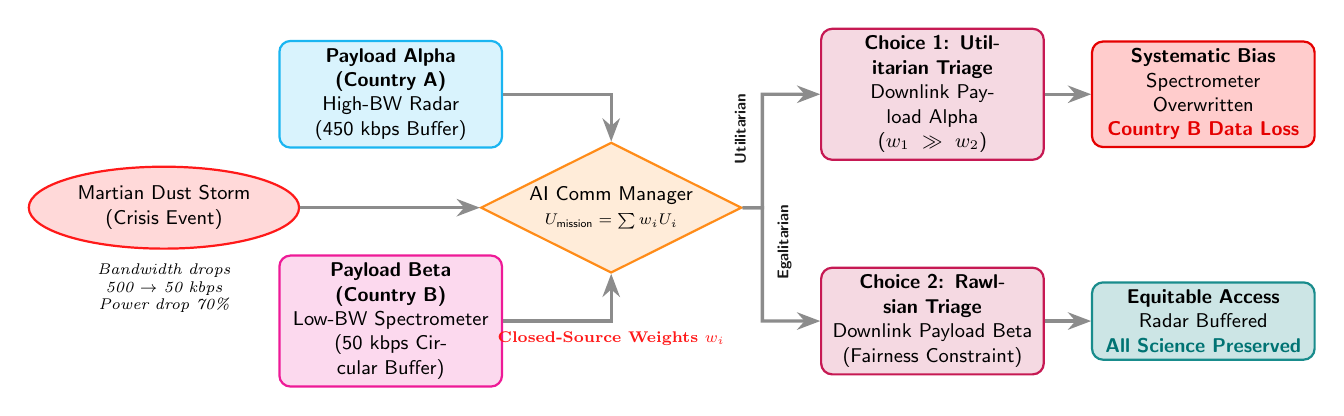
\begin{tikzpicture}[
    scale=0.8,
    transform shape,
    font=\sffamily\small,
    box/.style={
        rectangle, 
        draw=blue!90, 
        fill=blue!15, 
        thick, 
        rounded corners, 
        align=center, 
        minimum height=1.2cm,
        text width=3.3cm
    },
    crisis/.style={
        ellipse, 
        draw=red!90, 
        fill=red!15, 
        thick, 
        align=center,
        minimum height=1.0cm,
        text width=2.8cm
    },
    engine/.style={
        diamond, 
        draw=orange!90, 
        fill=orange!15, 
        thick, 
        align=center,
        aspect=2,
        minimum width=3.0cm,
        inner sep=1pt
    },
    decision/.style={
        rectangle, 
        draw=purple!90, 
        fill=purple!15, 
        thick, 
        rounded corners, 
        align=center, 
        minimum height=1.2cm,
        text width=3.3cm
    },
    outcomeRed/.style={
        rectangle, 
        draw=red!90!black, 
        fill=red!20, 
        thick, 
        rounded corners, 
        align=center, 
        minimum height=1.2cm,
        text width=3.3cm
    },
    outcomeTeal/.style={
        rectangle, 
        draw=teal!90, 
        fill=teal!20, 
        thick, 
        rounded corners, 
        align=center, 
        minimum height=1.2cm,
        text width=3.3cm
    },
    arrow/.style={
        thick, 
        -Stealth, 
        draw=gray!90,
        line width=1.2pt
    },
    labelstyle/.style={
        font=\sffamily\scriptsize\bfseries,
        color=black!90
    }
]
    % Level 1: Crisis Input
    \node [crisis] (storm) at (0,0) {Martian Dust Storm\\ (Crisis Event)};
    \node [below=0.1cm of storm, font=\scriptsize\itshape, text width=3.8cm, align=center] {Bandwidth drops 500 $\rightarrow$ 50 kbps\\ Power drop 70\%};

    % Level 2: Competing Inputs
    \node [box, draw=cyan!90, fill=cyan!15] (alpha) at (3.6, 1.8) {\textbf{Payload Alpha (Country A)}\\ High-BW Radar\\ (450 kbps Buffer)};
    \node [box, draw=magenta!90, fill=magenta!15] (beta) at (3.6, -1.8) {\textbf{Payload Beta (Country B)}\\ Low-BW Spectrometer\\ (50 kbps Circular Buffer)};

    % Level 3: Decision Engine
    \node [engine] (ai) at (7.1, 0) {AI Comm Manager\\ \scriptsize $U_{\text{mission}} = \sum w_i U_i$};
    \node [below=0.8cm of ai, font=\scriptsize\bfseries, color=red!90] {Closed-Source Weights $w_i$};

    % Level 4: Triage Decisions
    \node [decision] (pathA) at (12.2, 1.8) {\textbf{Choice 1: Utilitarian Triage}\\ Downlink Payload Alpha\\ ($w_1 \gg w_2$)};
    \node [decision] (pathB) at (12.2, -1.8) {\textbf{Choice 2: Rawlsian Triage}\\ Downlink Payload Beta\\ (Fairness Constraint)};

    % Level 5: Outcomes
    \node [outcomeRed] (outA) at (16.5, 1.8) {\textbf{Systematic Bias}\\ Spectrometer Overwritten\\ \color{red!90!black}\bfseries Country B Data Loss};
    \node [outcomeTeal] (outB) at (16.5, -1.8) {\textbf{Equitable Access}\\ Radar Buffered\\ \color{teal!90!black}\bfseries All Science Preserved};

    % Connections
    \draw [arrow] (storm.east) -- (ai.west);
    \draw [arrow] (alpha.east) -| (ai.north);
    \draw [arrow] (beta.east) -| (ai.south);
    
    \draw [arrow] (ai.east) -- (9.5, 0) -- (9.5, 1.8) node [midway, rotate=90, labelstyle, xshift=10pt, yshift=10pt] {Utilitarian} -- (pathA.west);
    \draw [arrow] (ai.east) -- (9.5, 0) -- (9.5, -1.8) node [midway, rotate=90, labelstyle, xshift=10pt, yshift=-10pt] {Egalitarian} -- (pathB.west);
    
    \draw [arrow] (pathA.east) -- (outA.west);
    \draw [arrow] (pathB.east) -- (outB.west);

\end{tikzpicture}
\end{document}
